\documentclass[UTF8]{ctexart}

\usepackage{WeeklyReport}
\usepackage{graphicx}
\usepackage{amsmath}
\usepackage{amssymb}

\title{周报08}
\author{傅阳烨}
\date{\today}

\begin{document}
    \maketitle
    % \tableofcontents
    \section{学习内容}
        \begin{itemize}
            \item 将前面看过的文章的思路迁移到 MSDA 的场景中
            \item 在 DomainNet 上训练和测试原模型和带 PAL 的模型
        \end{itemize}
    \section{学习收获}
        \subsection{将其它模型的思路迁移到 MSDA 中}
            \subsubsection{Teacher Student 和 Mutual Learning}
                把 Teacher Student 的想法放到 NPN 上,在原先的想法里,NPN 是一个反向更新的网络,
                带有 NPN 的网络往往效果会不如原网络,那么可以把原网络当作 Teacher,带 NPN 的网络当作 Student,
                当 Student 可以得到接近 Teacher 的正确率时,去掉 Student 的 NPN 网络进行测试。

                在 NPN 的权重较小的情况下,NPN 相当于是在 feature map 上添加了一层模糊层(或者是 noise 层),
                此时 Teacher Model 可以直接使用 Student 中 NPN 之外的网络(或者说 weight sharing)。
                使用 Teacher 输出的累积平均值或指数级累积平均值与 Student 的输出构成 Consistency Loss(论文中使用的是 Mean Square Difference)。

                把 Mutual Learning 迁移到 Multi-Source Domain Adaptation 上,对于两个网络的 Mutual Learning,训练的过程如下:

                使用交叉熵和KL散度衡量监督学习的loss和互学习的loss\footnote{如果是无监督学习,可以使用伪标签来计算交叉熵,而伪标签的生成可以使用原先看过的 Distilling 的方法}。

                对于某一个 class $m$ :

                $$
                    p_{1}^{m}(\boldsymbol{x}_i) = \frac{exp(z_{1}^{m})}{\sum_{m=1}^{M} exp(z_{1}^{m})}
                $$

                $$
                    L_{C_{1}} = - \sum_{i=1}^{N} \sum_{m=1}^{M} I(y_{i}, m) \log(p_{1}^{m}(\boldsymbol{x}_i))
                $$

                其中 $I$ 是一个 indicator function,当类标签 $y_i = m$ 时,值为 1,否则为 0。

                $$
                    D_{KL}(\boldsymbol{p}_{2}\|\boldsymbol{p}_{1}) = \sum_{i=1}^{N} \sum_{m=1}^{M} p_{2}^{m}(\boldsymbol{x}_i) \log \frac{p_{2}^{m}(\boldsymbol{x}_i)}{p_{1}^{m}(\boldsymbol{x}_i)}
                $$

                第一个网络的Loss可以写成:

                $$
                    L_{\Theta_{1}} = L_{C_{1}} + D_{KL}(\boldsymbol{p}_{2}\|\boldsymbol{p}_{1})
                $$

                第二个网络的Loss可以写成:

                $$
                    L_{\Theta_{2}} = L_{C_{2}} + D_{KL}(\boldsymbol{p}_{1}\|\boldsymbol{p}_{2})
                $$

                在训练的时候,交替迭代更新两个网络的参数。

                对于多源自适应的情况,提出两种训练思路:

                \begin{enumerate}
                    \item 在每个 epoch 中,每个 source domain 分别与 target 的网络进行参数更新(Mutual Learning),此时每个 Source Domain 是一个网络,target 也是一个网络
                    \item 直接构建多对 source-target 的组合进行 Mutual Learning,得到多个 target 的网络,在进行按一定权重(根据 source 和 target 之间的相关性进行权重设置)合并成一个网络,得到预测结果
                \end{enumerate}
            \subsubsection{Concrete Selector 和 Annealing Schedule}
                在 Concrete Selector 中,最主要的是一个 Concrete Distribution:

                $$
                    \mathbf{m}_j = \frac{\exp((\log \mathbf{\alpha}_j + \mathbf{g}_j)/T)}{\sum_{k=1}^d \exp((\log \mathbf{\alpha}_k + \mathbf{g}_k)/T)}
                $$

                其中 $\alpha \in \mathbb{R}^d_{>0}$ 是一个参数向量,$\textbf{g}_j$ 为 Grumble 分布的样本,$\mathbf{m}_j$ 表示的是某个样本向量中的第 $j$ 个元素。
                使用这个生成的向量 $m$ 去给 feature map 进行选择(或者说加权)。

                上述的过程相当于一个稀疏性会变化的线性组合,当 $T \rightarrow 0$ 时,得到的结果会接近 sparse。

                在训练的过程中,使用一个退火的公式去更新 $T$:

                $$
                    T(b) = T_0(\frac{T_B}{T_0})^{\frac{b}{B}}
                $$

                其中 $b$ 和 $B$ 分别表示当前训练的 epoch 和总的训练 epoch。

                在现在所做的多源领域适应模型中,这个 Concrete Selector Layer 可以直接放在 PAL 后面,
                把 PAL 的输出作为 $\alpha$ 向量输入到 Concrete Distribution 中,随着训练 Epoch 增加,特征选择的结果会越来越稀疏,
                达到选取共同特征的目的。
            \subsection{DomainNet 测试}
                这周把上周没写完的 DomainNet 训练代码完善了,但由于 hyper parameter 和训练模型都是直接套用了 DigitFive 的(论文没有给出 DomainNet 训练的超参和实现细节),
                而 DigitFive 本身分辨率很低,处理的时候是直接将 DomainNet 的原图放缩到与 DigitFive 数据集同样大小(节省训练时间,先得到初步的测试结果),
                再进行训练,效果上会有些下降。

                目前测试得到的结果如图 \ref{fig:test} 所示。

                \begin{figure}[ht]
                    \centering
                    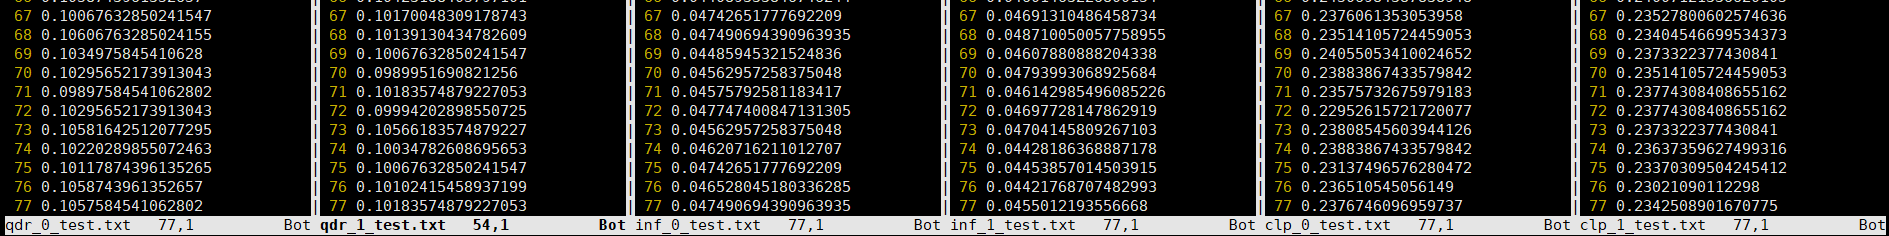
\includegraphics[scale=0.26]{Week08_DomainNet_test.png}
                    \caption{DomainNet 中 target 为 clipart、infograph 和 quickdraw 的测试,编号 0 为原模型的正确率,编号 1 为使用了 PAL 的模型的正确率}
                    \label{fig:test}
                \end{figure}

                在目标域为 clipart 和 infograph 的实验中,无论是原模型还是添加了 PAL 的模型,正确率都比论文中给出的正确率要低很多,由于没有怎么调整超参,以及图像放缩后非常模糊,所以这个结果也在预料之内。
                而在把 quickdraw 作为 target domain 的实验中,无论是原模型还是带 PAL 的模型,正确率都比文中给出的数据高 4\% 左右(仍然比其它模型的最高值低),
                可能是原作者在 quickdraw 这部分的实现有些问题。

                从结果上看,带 PAL 的模型比不带 PAL 的模型正确率反而下降了一些(约0.5\%),可能的原因在于超参没有设置好,
                直接将图像缩放到与 DigitFive 一样大可能会损失很多信息,并且训练的 epoch 少了一些,在最后几个 epoch 的时候,Loss1 和 Loss2 仍然维持在 1 以上,
                PAL 在 0.1 以上 (在 DigitFive 数据集上训练,这些 Loss 的数量级大约在 $10^{-2}$),相当于是在特征还没有提取出来或者特征还不正确的时候就进行了特征匹配,
                此时匹配后的特征可能并不能代表源域和目标域的共同特征。
    \section{改进思路}
        \begin{enumerate}
            \item 需要根据 DomainNet 调整 hyper parameter,如 learning rate、regularization 的权重,矩的阶数,数据 transform 时的均值和方差等,但由于接下来还需要在 DigitFive 上做别的方法的测试,所以这部分的超参暂时不改动
            \item 把原先的特征提取器和分类器(32 x 32)换成更大的特征提取器和分类器(如 200 x 300),保留原图的信息
            \item 增加训练的 epoch,在前面的实验中,模型并没有很好的收敛,训练结束时的 Loss 仍然比较大
        \end{enumerate}
    \section{疑问/困难}
        \begin{enumerate}
            \item 当前比较大的问题就是我自己实现的 DomainNet 测试结果比论文的结果要差很多,在训练的最后几个 Epoch,Loss 已经趋于稳定,但还是比较大。
            \item DomainNet 数据集中的类别很多(345个类),如果放缩到跟 DigitFive (10个类)同样的分辨率,所能提供的信息非常有限。在原作者所做的实验中也说明了类别增加确实会造成正确率下降,作者所公布的一些模型的测试结果,在 DomainNet 上的正确率大多在 40\% 以下,
                有的 target domain 甚至只有不到 20\%
        \end{enumerate}
\end{document}
